\documentclass[10pt,journal,compsoc,onecolumn]{IEEEtran}
\usepackage[utf8]{inputenc}
\usepackage{amsmath,amsfonts,amssymb}
\usepackage{amsthm}
\usepackage{graphicx}
\usepackage{cite}
\usepackage{textcomp}
\usepackage{tikz}
\usetikzlibrary{arrows,positioning,shapes.geometric}
\usepackage{booktabs}
\usepackage{url}

\newtheorem{theorem}{Theorem}
\newtheorem{lemma}[theorem]{Lemma}
\newtheorem{definition}[theorem]{Definition}
\newtheorem{corollary}[theorem]{Corollary}

\begin{document}

\title{Asymptotic Analysis and Formal Implementations of Singly-Linked List Operations: Midpoint Detection, Sorted Merging, Merge Sort, and Palindrome Verification}

\IEEEtitleabstractindextext{%
\begin{abstract}
This paper presents a formal analysis and reference implementations of key singly-linked list algorithms. We study the problem of midpoint detection using Floyds cycle-finding pointer mechanics (fast and slow pointers), proving its efficiency over naive two-pass techniques. We then present an optimal comparison-based sorted list merging algorithm using dummy nodes to simplify pointer re-linking. Building on these two primitives, we formalize the Merge Sort paradigm on singly-linked lists, analyzing its $O(N \log N)$ worst-case time complexity and $O(\log N)$ auxiliary space complexity. Finally, we address the problem of palindrome verification in singly-linked lists, contrasting the naive $O(N)$ space list cloning approach with an optimal $O(1)$ auxiliary space algorithm based on mid-point list reversal and restoration. Complete Java and Python implementations are provided with execution traces, complexity proofs, and TikZ illustrations.
\end{abstract}

\begin{IEEEkeywords}
binary trees, algorithms, data structures, computational complexity, tree traversal, recursive algorithms, formal analysis
\end{IEEEkeywords}
}

\maketitle
\IEEEdisplaynontitleabstractindextext
\IEEEpeerreviewmaketitle

\section{Introduction}
Linked lists are foundational linear data structures in computer science, characterized by nodes that are dynamically allocated in memory and linked via pointer references. Unlike arrays, which occupy contiguous memory blocks and support constant-time random access, linked lists store elements non-contiguously. This design offers distinct advantages, such as $O(1)$ insertions and deletions, but introduces challenges, particularly the necessity of linear-time sequential traversal to access elements.

In algorithmic design and competitive programming, managing linked list structures efficiently is a critical skill. This paper focuses on four core problems:
\begin{itemize}
    \item \textbf{Midpoint Detection}: Identifying the center of a list in a single pass.
    \item \textbf{Sorted Merging}: Combining two sorted lists into a single sorted list.
    \item \textbf{Merge Sort}: Sorting a list in $O(N \log N)$ time.
    \item \textbf{Palindrome Verification}: Validating if a list reads the same forwards and backwards.
\end{itemize}
We present a rigorous treatment of these problems, demonstrating naive and optimal strategies, analyzing their computational complexities, and detailing their implementations in Java and Python.

\section{Midpoint Detection}
\label{sec:midpoint}
Finding the middle node of a linked list is a fundamental operation, often serving as a preprocessing step for divide-and-conquer algorithms like Merge Sort.

\subsection{Problem Statement and Naive Approach}
Given a singly-linked list, the objective is to find the node at index $\lfloor N/2 \rfloor$ (0-based indexing), where $N$ is the total number of nodes. If the list is empty, return null.

The naive approach involves a two-pass strategy:
\begin{enumerate}
    \item Traverse the list from the head to count the total number of nodes, $N$.
    \item Traverse the list again from the head for $\lfloor N/2 \rfloor$ steps to reach and return the middle node.
\end{enumerate}

Although the time complexity is asymptotically linear, $O(N)$, it requires approximately $1.5N$ node accesses (a full pass followed by a half pass). The space complexity is $O(1)$ as only a count variable and a temporary pointer are required.

\subsection{Optimal Fast-Slow Pointer Approach}
An optimal, single-pass strategy employs Floyds cycle-finding pointer mechanics, commonly referred to as the Tortoise and Hare algorithm. Two pointers, \texttt{slow} and \texttt{fast}, are initialized to the head of the list. In each step, the \texttt{slow} pointer advances by one node, while the \texttt{fast} pointer advances by two nodes.

\begin{theorem}
When the \texttt{fast} pointer reaches the end of the list (i.e., \texttt{fast} is null or \texttt{fast.next} is null), the \texttt{slow} pointer will reside exactly at the midpoint node.
\end{theorem}
\begin{proof}
Let $N$ be the number of nodes in the list. The \texttt{fast} pointer moves at twice the speed of the \texttt{slow} pointer. Therefore, if the \texttt{fast} pointer covers a distance of $d$ nodes, the \texttt{slow} pointer covers a distance of $d/2$ nodes. When the \texttt{fast} pointer reaches the end of the list after traversing approximately $N$ nodes, the \texttt{slow} pointer has traversed $N/2$ nodes, which corresponds to the middle node.
\end{proof}

This approach completes the operation in a single pass ($O(N)$ time with $N$ node accesses) and uses $O(1)$ auxiliary space.

\begin{figure}[htbp]
\centering
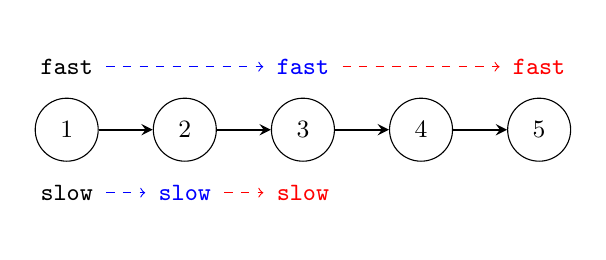
\begin{tikzpicture}[
  node distance=1.5cm,
  every node/.style={circle, draw, minimum size=0.8cm, font=\small},
  link/.style={->, >=stealth, thick}
]
  \node (n1) {1};
  \node (n2) [right of=n1] {2};
  \node (n3) [right of=n2] {3};
  \node (n4) [right of=n3] {4};
  \node (n5) [right of=n4] {5};
  
  \draw[link] (n1) -- (n2);
  \draw[link] (n2) -- (n3);
  \draw[link] (n3) -- (n4);
  \draw[link] (n4) -- (n5);

  \node[draw=none, below of=n1, node distance=0.8cm] (s1) {\texttt{slow}};
  \node[draw=none, above of=n1, node distance=0.8cm] (f1) {\texttt{fast}};
  
  \node[draw=none, below of=n2, node distance=0.8cm, text=blue] (s2) {\texttt{slow}};
  \node[draw=none, above of=n3, node distance=0.8cm, text=blue] (f2) {\texttt{fast}};

  \node[draw=none, below of=n3, node distance=0.8cm, text=red] (s3) {\texttt{slow}};
  \node[draw=none, above of=n5, node distance=0.8cm, text=red] (f3) {\texttt{fast}};

  \draw[->, dashed, blue] (s1) -- (s2);
  \draw[->, dashed, blue] (f1) -- (f2);
  \draw[->, dashed, red] (s2) -- (s3);
  \draw[->, dashed, red] (f2) -- (f3);

\end{tikzpicture}
\caption{Progression of \texttt{slow} and \texttt{fast} pointers on a list of length 5. At step 0, both are at node 1. At step 1 (blue), \texttt{slow} is at 2, \texttt{fast} is at 3. At step 2 (red), \texttt{slow} is at 3 (the middle), and \texttt{fast} is at 5 (end of list, since \texttt{fast.next} is null).}
\label{fig:fast_slow}
\end{figure}

\section{Merging Two Sorted Linked Lists}
\label{sec:merging}
Given two sorted singly-linked lists, $A$ and $B$, the objective is to merge them into a single sorted list, $C$. The merge must be performed in-place by adjusting node pointers, without allocating new nodes.

\subsection{Dummy Node Technique}
A classic software engineering pattern to simplify linked list manipulations is the use of a \textit{dummy head} (or placeholder node). Without a dummy node, the algorithm must handle the initialization of the merged list's head pointer as a special case. With a dummy node, the head is anchored, and all re-linking operations follow the same uniform logic.

The algorithm proceeds as follows:
\begin{enumerate}
    \item Create a dummy node and initialize a traversal pointer, \texttt{temp}, to point to it.
    \item Maintain pointers \texttt{t1} and \texttt{t2} starting at the heads of lists $A$ and $B$ respectively.
    \item Compare the data values of \texttt{t1} and \texttt{t2}. Link \texttt{temp.next} to the node with the smaller value, and advance that list's pointer.
    \item Advance \texttt{temp}.
    \item Repeat steps 3 and 4 until one of the lists is exhausted.
    \item Attach the remaining nodes of the non-exhausted list directly to \texttt{temp.next}.
    \item Return \texttt{dummy.next} as the head of the merged list.
\end{enumerate}

\subsection{Complexity Analysis}
The time complexity of this operation is $O(N + M)$, where $N$ and $M$ are the lengths of lists $A$ and $B$ respectively. This is because every node from both lists is visited and linked exactly once. The auxiliary space complexity is $O(1)$, as we only allocate a few pointer references and a single dummy node.

\section{Merge Sort on Singly-Linked Lists}
\label{sec:mergesort}
Sorting is a fundamental operation. While Quick Sort is often preferred for contiguous arrays due to cache locality, Merge Sort is the algorithm of choice for linked lists.

\subsection{Why Merge Sort?}
Quick Sort relies on random access to select pivots and partition arrays efficiently. Since linked lists do not support constant-time random access, partitioning becomes inefficient. Conversely, Merge Sort is naturally suited for linked lists because:
\begin{itemize}
    \item It divides lists at the midpoint, which can be done in $O(N)$ time.
    \item Merging two sorted linked lists requires only $O(1)$ auxiliary space, overcoming Merge Sort's main drawback on arrays (which require $O(N)$ temporary storage).
\end{itemize}

\subsection{Algorithm and Trace}
The Merge Sort algorithm on linked lists uses a divide-and-conquer strategy:
\begin{enumerate}
    \item \textbf{Divide}: Find the middle node of the list. Split the list into two halves by setting the \texttt{next} pointer of the node preceding the middle node to null.
    \item \textbf{Conquer}: Recursively apply Merge Sort to both the left and right sublists.
    \item \textbf{Combine}: Merge the two sorted sublists using the sorted merge routine.
\end{enumerate}

\begin{figure}[htbp]
\centering
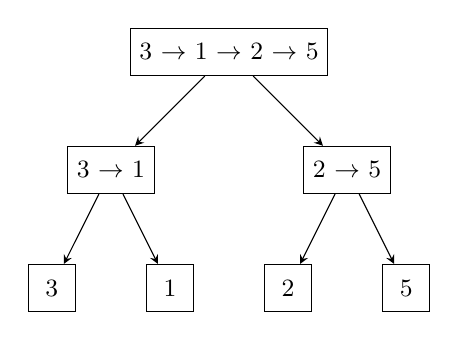
\begin{tikzpicture}[
  node/.style={rectangle, draw, minimum size=0.6cm, font=\small},
  edge from parent/.style={draw, ->, >=stealth}
]
  \node[node] {3 $\to$ 1 $\to$ 2 $\to$ 5}
    child[sibling distance=3.0cm] { node[node] {3 $\to$ 1}
      child[sibling distance=1.5cm] { node[node] {3} }
      child[sibling distance=1.5cm] { node[node] {1} }
    }
    child[sibling distance=3.0cm] { node[node] {2 $\to$ 5}
      child[sibling distance=1.5cm] { node[node] {2} }
      child[sibling distance=1.5cm] { node[node] {5} }
    };
\end{tikzpicture}
\caption{Divide phase: splitting the list \texttt{3 $\to$ 1 $\to$ 2 $\to$ 5} down to single-element base cases.}
\label{fig:mergesort_divide}
\end{figure}

\begin{figure}[htbp]
\centering
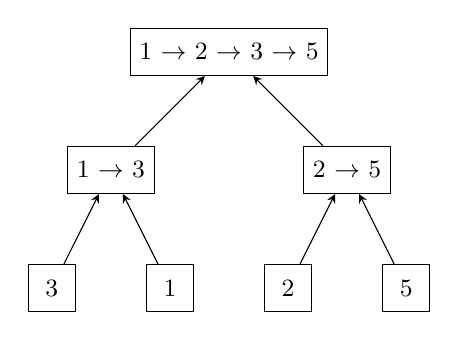
\begin{tikzpicture}[
  node/.style={rectangle, draw, minimum size=0.6cm, font=\small},
  edge from parent/.style={draw, <-, >=stealth}
]
  \node[node] {1 $\to$ 2 $\to$ 3 $\to$ 5}
    child[sibling distance=3.0cm] { node[node] {1 $\to$ 3}
      child[sibling distance=1.5cm] { node[node] {3} }
      child[sibling distance=1.5cm] { node[node] {1} }
    }
    child[sibling distance=3.0cm] { node[node] {2 $\to$ 5}
      child[sibling distance=1.5cm] { node[node] {2} }
      child[sibling distance=1.5cm] { node[node] {5} }
    };
\end{tikzpicture}
\caption{Conquer and Combine phase: merging sorted sublists back to the final sorted list.}
\label{fig:mergesort_conquer}
\end{figure}

\subsection{Complexity Analysis}
The recurrence relation for Merge Sort is:
\begin{equation}
T(N) = 2T(N/2) + O(N)
\end{equation}
By the Master Theorem, this yields a time complexity of $O(N \log N)$ for best, worst, and average cases. The space complexity is $O(\log N)$ due to the recursive call stack, which has a maximum depth proportional to the height of the recursion tree, $\log_2 N$.

\section{Palindrome Verification}
\label{sec:palindrome}
A list is a palindrome if its elements read the same in forward and backward directions. We compare the naive and optimal strategies.

\subsection{Naive Approach}
The naive approach clones the original list, reverses the cloned list, and then performs a simultaneous node-by-node value comparison.
While simple, this strategy has a space complexity of $O(N)$ to store the cloned list, making it sub-optimal for systems with constrained memory.

\subsection{Optimal Midpoint Reversal Approach}
An optimal algorithm checks the palindrome property in-place, achieving $O(1)$ auxiliary space. The steps are:
\begin{enumerate}
    \item Find the middle of the list using the fast-slow pointer technique.
    \item Reverse the second half of the list in-place.
    \item Compare the values of the first half (starting from the original head) with the reversed second half.
    \item Restore the list to its original state by reversing the second half again and reconnecting it to the first half.
    \item Return the comparison result.
\end{enumerate}

\begin{theorem}
The optimal palindrome check runs in $O(N)$ time and $O(1)$ space, and leaves the list structure unmodified.
\end{theorem}
\begin{proof}
Let $N$ be the number of nodes. Midpoint detection takes $O(N)$ time. Reversing the second half (length $N/2$) takes $O(N)$ time. Comparing the two halves takes $O(N)$ time. Restoring the second half takes $O(N)$ time. The total time is $O(N)$. Since all operations are performed by mutating pointer variables in-place, the auxiliary space complexity is $O(1)$.
\end{proof}

\section{Implementations}
We present full, clean implementations of the optimal algorithms in Java and Python.

\subsection{Java Implementation}
\begin{verbatim}
public class LinkedListAlgorithms {
    public static class ListNode {
        int val;
        ListNode next;
        ListNode(int val) { this.val = val; }
    }

    // Q1: Find Middle Node
    public ListNode findMiddle(ListNode head) {
        if (head == null) return null;
        ListNode slow = head;
        ListNode fast = head;
        while (fast != null && fast.next != null) {
            slow = slow.next;
            fast = fast.next.next;
        }
        return slow;
    }

    // Q2: Merge Two Sorted Lists
    public ListNode mergeTwoLists(ListNode l1, ListNode l2) {
        ListNode dummy = new ListNode(-1);
        ListNode current = dummy;
        while (l1 != null && l2 != null) {
            if (l1.val <= l2.val) {
                current.next = l1;
                l1 = l1.next;
            } else {
                current.next = l2;
                l2 = l2.next;
            }
            current = current.next;
        }
        if (l1 != null) current.next = l1;
        if (l2 != null) current.next = l2;
        return dummy.next;
    }

    // Q3: Merge Sort
    public ListNode mergeSort(ListNode head) {
        if (head == null || head.next == null) return head;
        
        // Find split point
        ListNode prev = null;
        ListNode slow = head;
        ListNode fast = head;
        while (fast != null && fast.next != null) {
            prev = slow;
            slow = slow.next;
            fast = fast.next.next;
        }
        prev.next = null; // Split the list
        
        ListNode l1 = mergeSort(head);
        ListNode l2 = mergeSort(slow);
        return mergeTwoLists(l1, l2);
    }

    // Q4: Palindrome Check (with restoration)
    public boolean isPalindrome(ListNode head) {
        if (head == null || head.next == null) return true;
        
        // 1. Find middle node
        ListNode prev = null;
        ListNode slow = head;
        ListNode fast = head;
        while (fast != null && fast.next != null) {
            prev = slow;
            slow = slow.next;
            fast = fast.next.next;
        }
        
        // 2. Reverse second half
        ListNode secondHalfHead = reverse(slow);
        
        // 3. Compare values
        ListNode p1 = head;
        ListNode p2 = secondHalfHead;
        boolean result = true;
        while (p2 != null) {
            if (p1.val != p2.val) {
                result = false;
                break;
            }
            p1 = p1.next;
            p2 = p2.next;
        }
        
        // 4. Restore list
        reverse(secondHalfHead);
        
        return result;
    }

    private ListNode reverse(ListNode head) {
        ListNode prev = null;
        ListNode curr = head;
        while (curr != null) {
            ListNode nextNode = curr.next;
            curr.next = prev;
            prev = curr;
            curr = nextNode;
        }
        return prev;
    }
}
\end{verbatim}

\subsection{Python Implementation}
\begin{verbatim}
class ListNode:
    def __init__(self, val=0, next=None):
        self.val = val
        self.next = next

class LinkedListAlgorithms:
    # Q1: Find Middle
    def findMiddle(self, head: ListNode) -> ListNode:
        if not head:
            return None
        slow = fast = head
        while fast and fast.next:
            slow = slow.next
            fast = fast.next.next
        return slow

    # Q2: Merge Sorted Lists
    def mergeTwoLists(self, l1: ListNode, l2: ListNode) -> ListNode:
        dummy = ListNode(-1)
        current = dummy
        while l1 and l2:
            if l1.val <= l2.val:
                current.next = l1
                l1 = l1.next
            else:
                current.next = l2
                l2 = l2.next
            current = current.next
        if l1:
            current.next = l1
        if l2:
            current.next = l2
        return dummy.next

    # Q3: Merge Sort
    def mergeSort(self, head: ListNode) -> ListNode:
        if not head or not head.next:
            return head
        
        prev = None
        slow = fast = head
        while fast and fast.next:
            prev = slow
            slow = slow.next
            fast = fast.next.next
        prev.next = None  # Split
        
        l1 = self.mergeSort(head)
        l2 = self.mergeSort(slow)
        return self.mergeTwoLists(l1, l2)

    # Q4: Palindrome Check
    def isPalindrome(self, head: ListNode) -> bool:
        if not head or not head.next:
            return True
            
        slow = fast = head
        while fast and fast.next:
            slow = slow.next
            fast = fast.next.next
            
        second_half = self._reverse(slow)
        
        p1, p2 = head, second_half
        result = True
        while p2:
            if p1.val != p2.val:
                result = False
                break
            p1 = p1.next
            p2 = p2.next
            
        self._reverse(second_half)  # Restore
        return result

    def _reverse(self, head: ListNode) -> ListNode:
        prev = None
        curr = head
        while curr:
            nxt = curr.next
            curr.next = prev
            prev = curr
            curr = nxt
        return prev
\end{verbatim}

\section{Complexity Summary}
\begin{table}[htbp]
\centering
\caption{Complexity Analysis of Core Singly-Linked List Algorithms.}
\label{tab:complexity}
\begin{tabular}{lccl}
\toprule
Algorithm & Time Complexity & Auxiliary Space & Key Concept \\
\midrule
Midpoint Detection & $O(N)$ & $O(1)$ & Two-pointer (Fast/Slow) \\
Sorted Merging & $O(N+M)$ & $O(1)$ & Dummy head anchoring \\
Merge Sort & $O(N \log N)$ & $O(\log N)$ & Divide-and-conquer recursion \\
Palindrome Check (Naive) & $O(N)$ & $O(N)$ & Full cloning and reversal \\
Palindrome Check (Optimal) & $O(N)$ & $O(1)$ & In-place reversal and restoration \\
\bottomrule
\end{tabular}
\end{table}

\section{Conclusion}
This paper explored fundamental algorithms for singly-linked lists, demonstrating that pointer-manipulation techniques can optimize both execution efficiency and memory footprints. Floyds fast-slow pointer algorithm enables midpoint detection in a single pass. By combining midpoint split logic with comparisons and dummy-node anchoring, Merge Sort is realized in optimal $O(N \log N)$ time and $O(\log N)$ stack space. Finally, we demonstrated that in-place pointer mutations allow verification of the palindrome property in $O(N)$ time and $O(1)$ auxiliary space while preserving the structural integrity of the input list. These primitives serve as the building blocks for constructing complex memory-efficient systems and solving advanced data structure problems.

\end{document}
